\chapter{Methods}

In this chapter we describe the methods we implement and compare in this thesis. All of them are block pruning methods (Section \ref{sec:block_pruning}) that permute a dimension of the score matrix to reduce the aggregated score of the pruned elements, and differ only in how this permutation is found.

In Chapter \ref{chap:preliminaries} we described TETRIS in its full generality as an algorithm over a $d$-dimensional weight tensor with $d$ separate permutations $\alpha_1, \ldots, \alpha_d$. For the remainder of this thesis we specialize to the 2D matrix case with \emph{slice blocks} of shape $1 \times k$ for a fixed $k$ (e.g., $1 \times 2$ or $1 \times 4$), where $k$ is assumed to divide the number of columns of the score matrix. Under this specialization only the column permutation is relevant; we denote it simply by $\pi$.

All methods take as input a score matrix $S$ (for instance, the entrywise absolute values of the weight matrix $|W|$, or Wanda scores $S_{ij} = (W_{ij} \|X_j\|)^2$) and produce a column permutation $\pi$ minimizing the entrywise $L_1$ norm of the pruned submatrix:
$$ \pi^* = \arg\min_{\pi} \sum_{(i,j) \in \text{pruned}} \big|S_{i,\pi(j)}\big|. $$
In typical use cases --- including all importance metrics considered in this thesis --- $S$ is non-negative by construction, so the absolute value becomes a formality and the objective reduces to a plain sum of pruned scores.

\section{Sort one dimension}
TODO: 12.4.

\section{Original TETRIS}
\label{sec:original_tetris}

We implemented the TETRIS algorithm described in Section \ref{sec:tetris} adapted to the 2D matrix case with $1 \times k$ slice blocks outlined in the introduction of this chapter. Since only the column permutation is relevant, the $d$-dimensional contraction from Section \ref{sec:tetris} collapses to a single step. Given the current permuted score matrix $S[\,:,\pi]$ and the block mask $M$ computed from it, we form
$$ C_{ij} = \sum_{k} \big|S_{k, \pi(i)}\big| \cdot M_{k, j}, $$
where $C_{ij}$ is the $L_1$ mass of the unpruned entries that column $\pi(i)$ would contribute if placed at position $j$. The gain matrix follows the definition from Section \ref{sec:tetris},
$$ G = L + L^\top - C - C^\top, $$
where $L$ is the diagonal of $C$ broadcast to a full matrix. The entry $G_{ij}$ quantifies the decrease in pruned $L_1$ mass obtained by swapping columns at positions $i$ and $j$ in the current permutation.

The reordering then proceeds greedily. At each step, the algorithm identifies the pair $(i, j)$ with the largest positive gain $G_{ij}$ and applies the corresponding swap to $\pi$. After every swap the mask $M$ and the gain matrix $G$ are recomputed, since both depend on the current column arrangement. The procedure terminates when no swap yields a positive gain, i.e. when $\max_{i,j} G_{ij} \leq 0$, indicating that the permutation is a local optimum of the objective under pairwise swaps.

\begin{lstlisting}[style=pseudocode,
                   caption={Original TETRIS (1D column specialization)},
                   label={alg:original_tetris}]
Input:  Score matrix $S \in \mathbb{R}^{m \times n}$, sparsity $s$, block shape $(1, k)$
Output: Column permutation $\pi$

$\pi \leftarrow (1, 2, \ldots, n)$
Repeat
    $M \leftarrow \mathrm{block\_mask}(S[:, \pi],\, s,\, (1,k))$
    $G \leftarrow \mathrm{gain\_matrix}(S[:, \pi],\, 1 - M)$
    $(i, j) \leftarrow \arg\max_{i',j'} G_{i',j'}$
    if $G_{i,j} > 0$ then swap $\pi_i$ and $\pi_j$
Until $\max_{i,j} G_{ij} \leq 0$
Return $\pi$
\end{lstlisting}

A step-by-step visualization of one iteration of the algorithm is shown in Figure \ref{fig:tetris_iteration}.

\begin{figure}[h]
    \centerline{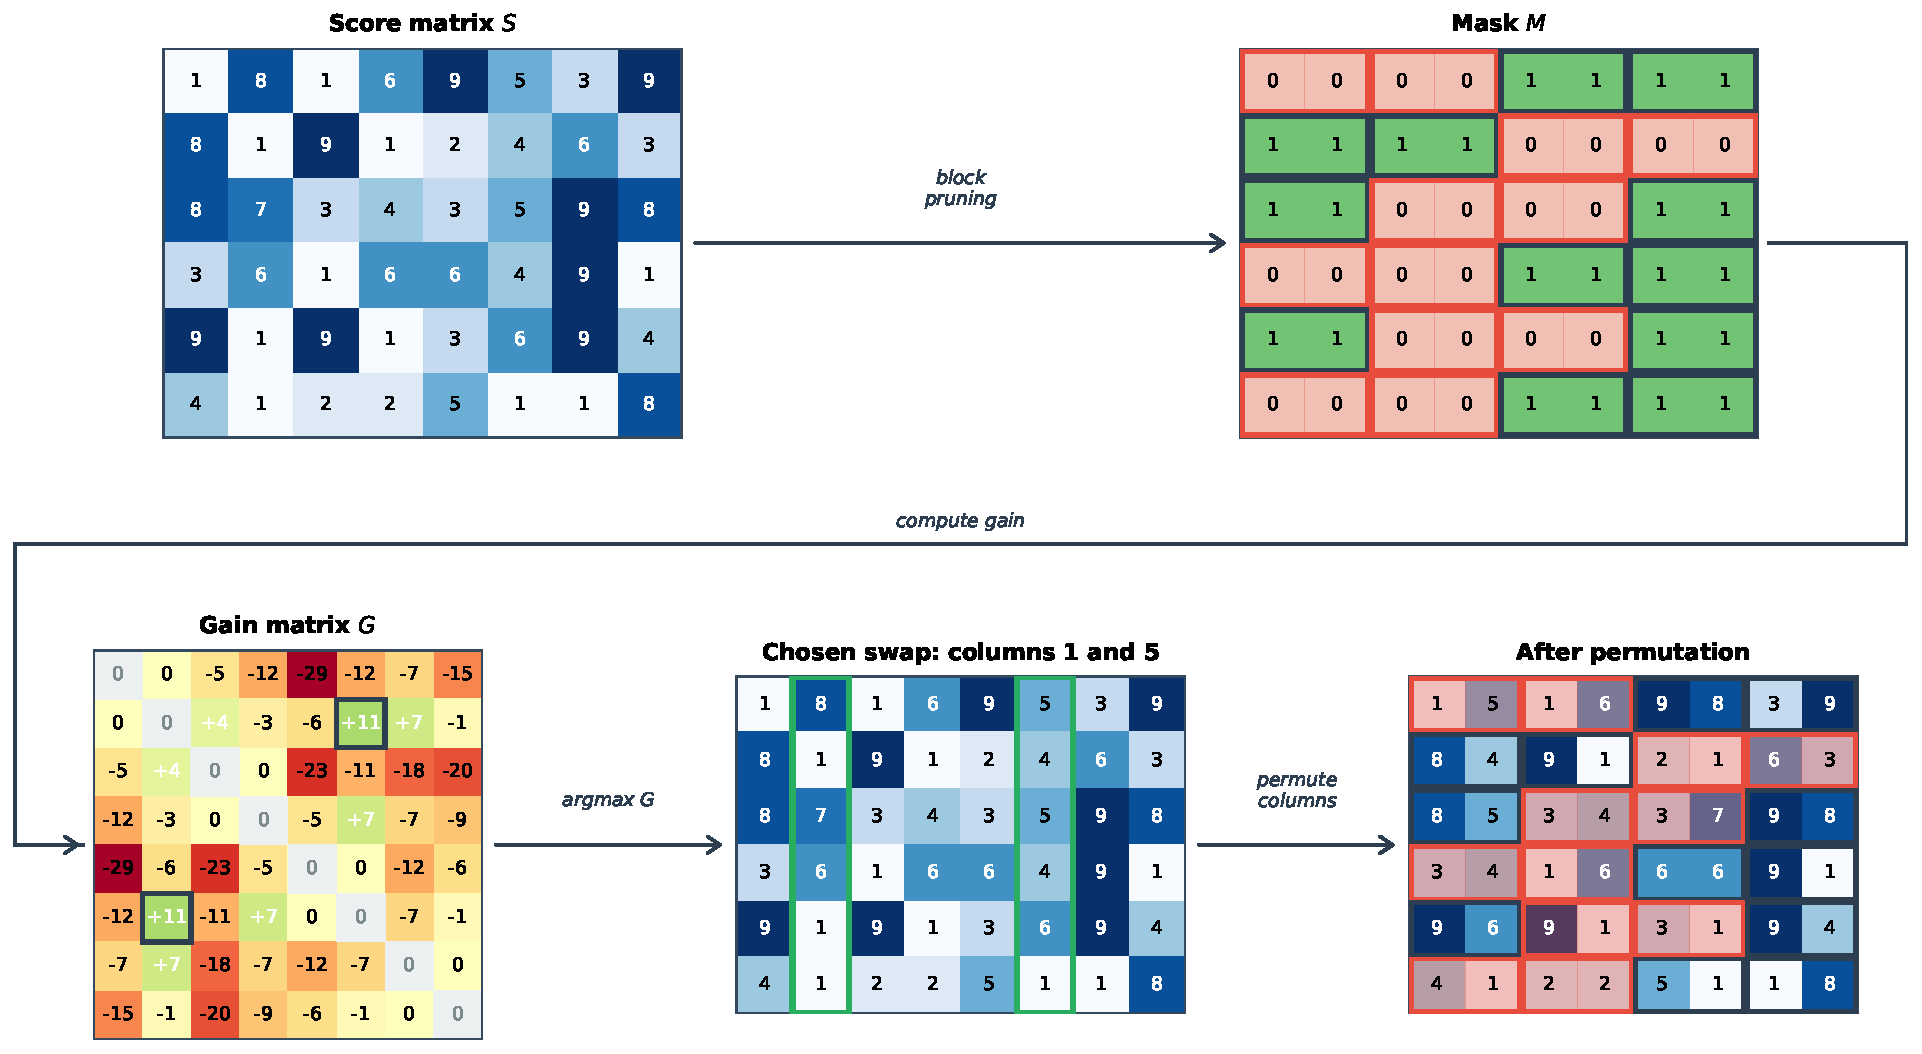
\includegraphics[width=1\textwidth]{images/tetris_iteration}}
    \caption[One iteration of TETRIS]{One iteration of the TETRIS algorithm: score matrix -> mask -> gain matrix -> chosen swap -> new permutation.}
    \label{fig:tetris_iteration}
\end{figure}

Since the algorithm only accepts swaps that decrease the objective, it is guaranteed to converge in a finite number of steps. The downside is that it gets stuck at the first local optimum it reaches, with no way to escape toward permutations that would require a more complex rearrangement to reach. The following section describes our method, which replaces this greedy step with an exact assignment solution.


\section{Global Assignment TETRIS}
\label{sec:ga_tetris}

The greedy search in original TETRIS explores only local moves. Most permutations are not reachable by a single swap, and once the greedy search stops at the first local optimum, it has no way of moving on to better permutations that would require a more complex rearrangement.

In this section we show that for a \emph{fixed} mask $M$, finding the optimal column permutation can be reformulated as a classic combinatorial optimization problem --- the maximum-weight perfect matching in a bipartite graph --- which can be solved exactly in polynomial time. We refer to this variant as \textit{Global Assignment TETRIS}, abbreviated \textit{GA-TETRIS}, reflecting the algorithmic substitution at its core: the local single-swap is replaced by a global reassignment of all columns at once.

\subsection*{Permutations as bipartite matchings}
\label{sec:permutation_as_matching}

Any permutation of $n$ elements can be represented as a perfect matching in a complete bipartite graph $K_{n,n}$. Let $A = \{a_1, \ldots, a_n\}$ and $B = \{b_1, \ldots, b_n\}$ be the two vertex sets, each indexed by column positions. A permutation $\pi$ is encoded by the set of edges $\{(a_i, b_{\pi(i)}) : i = 1, \ldots, n\}$: the edge $(a_i, b_j)$ is included whenever $\pi(i) = j$, i.e. when the column originally at position $i$ is moved to position $j$. Every permutation yields a perfect matching, and every perfect matching in $K_{n,n}$ encodes a unique permutation. Figure \ref{fig:permutation_graph} shows the perfect matching in the bipartite graph for the permutation $[2, 4, 1, 3, 5]$.

\begin{figure}[h]
    \centerline{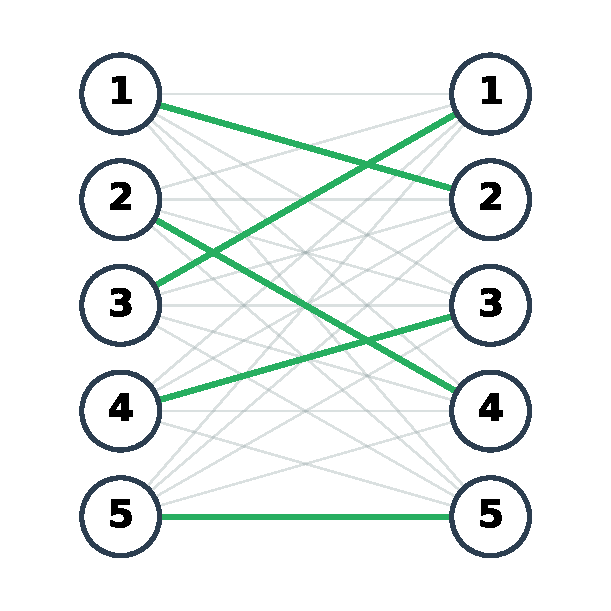
\includegraphics[width=0.8\textwidth]{images/permutation_graph}}
    \caption[Bipartite graph representing a permutation]{The bipartite graph $K_{5,5}$ with the perfect matching corresponding to the permutation $[2, 4, 1, 3, 5]$ highlighted.}
    \label{fig:permutation_graph}
\end{figure}
TODO: lepsi obrazok, porazi ma z tychto zakrut :D a mozno pridat nejakou sivou vsetky hrany a potom to mozem nazvat kompletny graf

\subsection*{From permutation objective to matching weight}

To turn this representation into an optimization problem, we need edge weights whose sum along a matching reflects how good the corresponding permutation is. We reuse the gain matrix $G$ defined in Section \ref{sec:tetris}: given the current permuted score matrix and mask $M$, the entry $G_{ij}$ measures the decrease in pruned $L_1$ mass obtained by swapping columns at positions $i$ and $j$. We assign this value as the weight of edge $(a_i, b_j)$. The resulting weighted bipartite graph is illustrated in Figure \ref{fig:weighted}.

\begin{figure}[h]
    \centerline{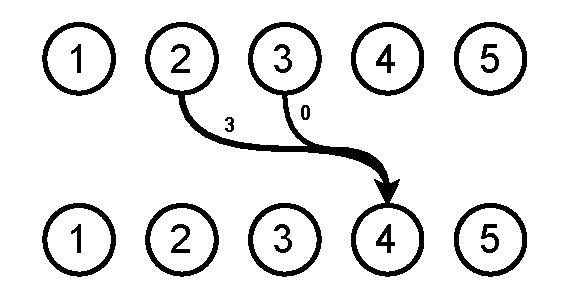
\includegraphics[width=0.8\textwidth]{images/weighted}}
    \caption[Weighted bipartite graph]{The weighted bipartite graph corresponding to a step of the reordering algorithm. Each edge carries the entry $G_{ij}$ of the gain matrix.}
    \label{fig:weighted}
\end{figure}
TODO: tu treba lepsi obrazok o dost

The total weight of a matching is then $\sum_i G_{i, \pi(i)}$. Under this correspondence, the maximum-weight perfect matching is the permutation that most reduces the pruning objective, as measured by $G$.

\subsection*{Reduction to the linear assignment problem}

Finding the maximum-weight perfect matching in a bipartite graph is equivalent to the \emph{linear assignment problem}, which is solved by the Hungarian algorithm \cite{kuhn1955hungarian}; an $O(n^3)$ refinement was later given by Edmonds and Karp \cite{edmonds1972theoretical}. We use the implementation provided by \texttt{scipy.optimize.linear\_sum\_assignment} \cite{scipy, crouse2016hungarian} that also runs in $O(n^3)$ time.

One important detail: the mask itself depends on how the columns are arranged, so solving the assignment problem once only gives us the best permutation for the current mask, not the best overall. To address this, we reuse the iterative structure of the original TETRIS. In each iteration, we recompute the mask from the current permuted matrix, solve the assignment problem against this updated mask, and apply the resulting permutation. The loop then continues for a fixed number of iterations.
